% LIGO background
The Advanced LIGO~\cite{TheLIGOScientific:2014jea} gravitational-wave detector network has completed three observing runs to date, searching the universe for astrophysical signals from coalescing binary systems, spinning neutron stars, and core-collapse supernovae. The first observing run saw the first direct detection of gravitational waves from the binary black hole merger GW150914~\cite{Abbott:2016blz}. The Virgo detector~\cite{TheVirgo:2014hva} joined the network towards the end of the second observing run, and on August 17, 2017 the first signal from a binary neutron star merger was observed~\cite{TheLIGOScientific:2017qsa}. The aftermath of this binary neutron star merger was observed across the entire electromagnetic spectrum~\cite{GBM:2017lvd}, from gamma-rays to radio, providing an unprecedented window onto the dynamics of these events. The full catalog of confident detections to date stands at 52 signals~\cite{LIGOScientific:2018mvr,LIGOScientific:2020ibl}, including two from binary neutron stars, two probable neutron star--black hole systems~\cite{LIGOScientific:2021qlt}, and a binary system whose secondary compact object is either the highest mass neutron star or the lowest mass black hole ever observed~\cite{LIGOScientific:2020zkf}. With the next observing runs of the current detector network promising significantly improved sensitivity~\cite{Aasi:2013wya}, and planning well underway for the third-generation detectors Cosmic Explorer~\cite{Reitze:2019iox} and Einstein Telescope~\cite{Punturo:2010zz}, the coming decades will provide an incredible opportunity to improve our understanding of neutron stars, black holes, and fundamental physics. In this thesis, we use observations of binary neutron star mergers to study the properties of neutron stars. We also examine the ability of current and future gravitational-wave detectors to measure the nuclear equation of state which describes the behavior of the high density nucleonic matter that makes up the interior of a neutron star.

\section{Gravitational-wave detectors}
The two Advanced LIGO detectors, located in Hanford, Washington and Livingston, Louisiana, together with the Virgo detector in Cascina, Italy comprise a worldwide gravitational-wave detector network. These detectors are Michelson interferometers with a Fabry-Perot cavity in each arm which stores the laser light for $\sim 100$ bounces, increasing the apparent arm length by two orders of magnitude. As a gravitational-wave passes through the detector it causes space-time to be stretched and squeezed. In an interferometric gravitational-wave detector this distortion results in small changes in the lengths of the arms. This change in arm length is measured as a phase difference over time in the laser light that is recombined from both arms, which allows the measurement of a passing gravitational wave.

Gravitational-wave detectors measure signal amplitude in terms of dimensionless ``strain" $h$, which is given by
\begin{equation}\label{eqn:intro_strain}
    h = \frac{\Delta L}{L} ,
\end{equation}
where $L$ is the arm length of the detector and $\Delta L$ is the change in arm length induced by the source. The sensitivity of the detectors is determined by a combination of noise sources including environmental, thermal, and quantum noise, among others~\cite{Martynov:2016fzi}. Each noise source impacts detector sensitivity in particular frequency bands, e.g. environmental noise includes seismic motion which limits detector sensitivity at frequencies $\lesssim 10$~Hz, and quantum noise includes uncertainty in the photon arrival time which can be interpreted as shot noise and suppresses sensitivity at frequencies $\gtrsim 200$~Hz. The overall sensitive band for the LIGO and Virgo detectors is roughly $15-1000$~Hz. From Eqn.~\ref{eqn:intro_strain} it can be seen that detector sensitivity increases with arm length $L$. To take advantage of this, the LIGO detectors were designed with 4~km arms and the Virgo detector has 3~km arms. Cosmic Explorer is a planned third-generation detector which will use the same general design as the LIGO and Virgo detectors except it will have 40~km arms. By increasing the arm lengths by an order of magnitude as compared to the LIGO detectors, Cosmic Explorer will have roughly an order of magnitude greater sensitivity. In Fig.~\ref{fig:intro_noise_curves} we show the noise curves for the LIGO detectors in the most recent observing run, as well as planned upgrade stages and a number of proposed detectors.

\begin{figure}[ht]
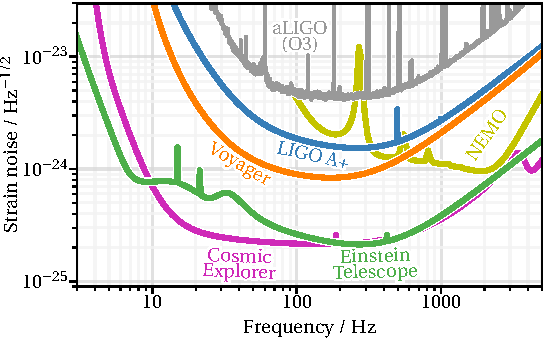
\includegraphics[width=\textwidth]{Figures/Introduction/asd_curves.pdf}
\caption{Noise curves, plotted as the amplitude spectral density, for the LIGO detectors in the most recently completed observing run (aLIGO) as well as a selection of proposed upgrade stages and future detectors. LIGO A+ is a planned upgrade to the LIGO detectors which will include improved quantum squeezing and mirror coatings. Voyager is a planned detector featuring a new design in the existing LIGO facilities, which will operate with a laser of 2 micron wavelength. NEMO is a proposed Australian detector optimized for high frequency sensitivity to study neutron star physics~\cite{Ackley:2020atn}. Cosmic Explorer is a planned third-generation detector similar in design to the LIGO detectors except with 40~km arms. Einstein Telescope is another planned third-generation detector which will be located underground, with 10~km arms in an equilateral triangle configuration.}
\label{fig:intro_noise_curves}
\end{figure}

\section{Multimessenger astrophysics}
The first observed binary neutron star merger GW170817 was also the first ``multimessenger" gravitational-wave event, as it was observed with both gravitational and electromagnetic waves: a short gamma-ray burst was observed $\sim 2$ seconds after the gravitational-wave signal~\cite{Goldstein:2017mmi,Savchenko:2017ffs}, and subsequent electromagnetic emission at X-ray, ultraviolet, optical, infrared, and radio frequencies identified a two-component kilonova~\cite{Chornock:2017sdf,Cowperthwaite:2017dyu,Kasliwal:2017ngb,Nicholl:2017ahq,Pian:2017gtc,Smartt:2017fuw,Villar:2017wcc}. Detection of an electromagnetic counterpart enables better understanding of the nature of the merger event and the properties of the neutron stars involved. One example of the benefit of multimessenger information is to break the distance-inclination degeneracy that is present in the amplitude of a gravitational-wave signal from a binary merger. This degeneracy arises from the fact that the gravitational-wave emission is strongest parallel or anti-parallel to the direction of the orbital angular momentum of the binary~\cite{Wahlquist:1987rx}, as a result of the amplitude of the two polarizations of the gravitational wave being maximum in these directions~\cite{Usman:2018imj}. Thus the inclination of the orbital plane is degenerate with the distance to the source, where a more face-on (or face-away) orientation of the binary at a larger distance is degenerate with a binary that is closer, but less well-aligned.

In Ch.~\ref{ch:inc-angle} we present an analysis of GW170817 informed by electromagnetic distance measurements of its identified host galaxy, NGC~4993~\cite{Soares-Santos:2017lru}. We demonstrate that using an independent distance measurement in a gravitational-wave analysis can break the distance-inclination degeneracy to allow for much tighter constraints on the inclination angle of the orbital plane of the binary with respect to the line of sight. We present our measurement in the context of the timing delay of the gamma-ray burst and observations of the long-lived kilonova afterglow emission to discuss implications for jet models.

With the increased sensitivity of the next observing runs and future detectors, we expect significantly more potential multimessenger events in the coming years, such that it will be necessary for gravitational-wave parameter estimation analyses to complete in a short amount of time to enable efficient prioritization of resources for electromagnetic follow-up observations~\cite{Margalit:2019dpi}. However, the measurement of source parameters for low-mass binary inspirals, such as binary neutron star or neutron star--black hole mergers, is very computationally expensive as a result of the long duration of these signals in the sensitive band of gravitational-wave detectors: a typical binary neutron star signal entering the sensitive band at 20~Hz will last several minutes before merging. At a sample rate of 4096~Hz, which is standard for most parameter estimation analyses, this translates to $\sim 2 \times 10^5$ frequency-domain data samples required to capture the signal. Each evaluation of the likelihood then requires a frequency-domain inner-product of this detector data with a template waveform, and a full parameter estimation analysis can require $\mathcal{O}(10^9)$ likelihood evaluations~\cite{Biwer:2018osg}. Several methods have been developed to help reduce computational cost~\cite{Purrer:2014fza,Canizares:2014fya,Blackman:2014maa,Purrer:2015tud,Field:2013cfa,Caudill:2011kv,Field:2011mf,Canizares:2013ywa,Blackman:2015pia}. In this thesis we focus on the ``relative binning" technique, which uses an approximation to the likelihood near its peak in order to allow the use of fewer frequency samples in each likelihood calculation~\cite{cornish2013fast,Zackay:2018qdy}.

In Ch.~\ref{ch:rel-bin-pe} we present an implementation of the relative binning parameter estimation technique as a likelihood model in \textit{PyCBC Inference}. We extend the relative model to a coherent network statistic to allow sky localization, and we enable use for any frequency-domain waveform approximant available in LALSuite~\cite{2020ascl.soft12021L}. We validate the relative model on large simulated populations of binary neutron star and neutron star--black hole signals. We demonstrate the feasibility of seeding the analysis of each simulated signal with the best-fit template parameters from a low latency search pipeline, showing the real-world utility of this model in producing fast and accurate parameter estimates that can be used to inform electromagnetic follow-up observations.

\section{Nuclear equation of state}
Neutron stars contain matter at some of the highest densities in the known universe, therefore they can serve as astrophysical laboratories to study how matter behaves under these extreme conditions. The behavior of this dense matter is described by the nuclear equation of state. Gravitational waves from a binary neutron star merger will carry information about the nuclear equation of state through the tidal deformability $\Lambda$ of the neutron stars: as the pair of neutron stars inspiral and their orbital separation decreases, the gravitational field of each star will induce a deformation in the body of its companion. This tidal deformation is measurable in a gravitational-wave signal as the energy required to induce the effect alters the gravitational-wave phase evolution of the inspiral~\cite{Flanagan:2007ix}. 

The gravitational waveforms used to measure the nuclear equation of state are computed using either post-Newtonian methods, which
are perturbative expansions in the invariant velocity of the binary, or
using effective-one-body models that include tidal
effects~\cite{Damour:2009wj,Bini:2012gu,Bernuzzi:2014owa,Hotokezaka:2015xka,Nagar:2018plt,Akcay:2018yyh} 
and provide better accuracy than post-Newtonian models by tuning higher-order
terms to numerical relativity waveforms. 
The post-Newtonian waveform is written as a power series in the invariant velocity $v = (\pi M f)^{1/3}$, where $f$ is the gravitational-wave frequency and $M = m_1 + m_2$ is the total mass of the binary. As $v$ increases throughout the inspiral, the 
tidal terms become large enough to contribute a measurable phase shift in the gravitational-wave signal. Since the tidal deformation only becomes significant for small orbital separations, the effect in the gravitational-wave signal is only measurable at the higher frequencies just before merger. It has been found that tidal effects only become important for frequencies $f \gtrsim 400$~Hz~\cite{Harry:2018hke}. Gravitational-wave detectors that use a laser interferometer are generally less sensitive at these higher frequencies as a result of quantum noise~\cite{Caves:1981hw}, making tidal effects challenging to measure. 

In Ch.~\ref{ch:common-radius} we perform the first open-data analysis of GW170817 focused on measuring the tidal deformability of the merging neutron stars. We impose a physical constraint requiring that both neutron stars obey a common equation of state, and we construct a prior on the leading order tidal parameter that is uniform to reflect our uninformed prior knowledge. We describe the derivation of our constraint and present measurements of the tidal deformability and neutron star radius under several different assumptions about the mass distribution of neutron stars in merging binaries. 

A number of previous studies have examined Advanced LIGO's ability to measure the neutron star equation of state through the star's tidal deformability. Lackey \textit{et al.} \cite{Lackey:2014fwa} performed parameter estimation for the loudest twenty binary neutron star events in a year of data, with signal-to-noise ratios ranging from 13 to 64 in Advanced LIGO at design sensitivity. They found that only the loudest five events are the most informative toward constraining the equation of state. To constrain the equation of state they measure the tidal deformability parameter $\tilde{\Lambda}$, which is the linear combination of the individual tidal parameters $\Lambda_1$ and $\Lambda_2$. 
%They claim that including prior information for $\tilde{\Lambda}$ is easier than it is for a $\lambda(m)$ fit for the equation of state. 
To combine the information from multiple events, they follow a two-step process. First, they sample the posteriors for each of the events individually and then marginalize over all the parameters except the equation of state dependent parameters (i.e. $m_1, m_2, \tilde{\Lambda}$) to obtain a quasilikelihood. In the second step they sample the joint likelihood for $n$ binary neutron star events, taking into account that $\tilde{\Lambda}$ can be expressed in terms of the masses and the equation of state parameters, and then marginalize over the masses. They also use Fisher matrix analysis for high signal-to-noise ratio events to compute the quasilikelihood, and find that for the most part the results with Fisher matrix are comparable to the Bayesian analysis, but that they slightly underestimate the uncertainty in  radius, pressure and tidal deformability. They find that when stacking events together, the statistical error reduces, but the systematic error remains. They claim that systematic errors are due to uncertainties in the post-Newtonian waveform models.

Agathos \textit{et al.} \cite{Agathos:2015uaa} expand on the work by Ref.~\cite{Lackey:2014fwa} by including more events, spins for the neutron stars, and by terminating the waveforms at the first point of contact. They also include higher post-Newtonian terms  in their waveform model. They attempt to infer the neutron star equation of state via two methods: hypothesis ranking and parameter estimation. For hypothesis ranking, they evaluate the odds ratio and rank the equations of state. The highest ranked equation of state is assumed to be the one that is closest to the true equation of state. For parameter estimation, they expand the $\Lambda (m)$ relation around $m_0 = 1.4$\msun\ at quadratic order. This allows them to combine the equation of state dependent parameters for multiple detections, which are the coefficients $c_j$ in the quadratic expression for $\Lambda (m)$. For the signals they use, they are only able to measure $c_0$ and can't infer $c_1$, $c_2$. Their signals have signal-to-noise ratio between 8 and 30. They find that more than 50 sources are needed to make comparative equation of state studies successful for the equations of state that they examine. They also find that if the source mass distribution is strongly peaked, using flat priors while inferring the equation of state parameters induces systematic errors. They suggest that this can be mitigated by including better priors for the masses by incorporating information on masses from other astrophysical observations. Unfortunately, the equations of state examined by Agathos \textit{et al.} are quite stiff (i.e. have a large radius for a given mass), and they are disfavored by GW170817. Since the measurability of the tidal deformability depends on the nuclear equation of state, with stiffer equations being easier to probe as they produce a larger gravitational-wave phase shift, the results of Agathos \textit{et al.} are overly optimistic in light of current knowledge.

More recent work has extended the above analyses using the Fisher matrix formalism, and the inclusion of measurements of the equation of state by other independent methods such as from \textit{NICER}. Forbes \textit{et al.} \cite{Forbes:2019xaz} perform Fisher matrix analysis for low signal-to-noise ratio events while parameterizing the equation of state with 18 different parameters. They claim that a handful of events will be able to significantly constrain the equation of state. Similarly, Carson \textit{et al.} \cite{Carson:2019rjx} use a Fisher matrix analysis to explore the implications of multiple binary neutron star detections with current and future generation detectors to determine the uncertainty in measuring the tidal deformability. They claim that the uncertainties will continue to dominate until the end of Voyager-type detectors. 

Recently, Landry \textit{et al.} \cite{Landry:2020vaw} studied the equation of state constraints from multiple gravitational wave observations, \textit{NICER} observations, and including information from the detection of the most massive neutron stars observed as radio pulsars. They estimate $\sim 60$ total events by the end of Advanced LIGO's fourth observing run, and $\sim 4$ events with signal-to-noise ratio $\geq 20$. They claim that with multiple binary neutron star events by the end of Advanced LIGO's fifth observing run, and including the \textit{NICER} and radio observations, tight constraints can be placed on the equation of state. They find that the uncertainty in the tidal deformability of a 1.4\msun\ neutron star $\Delta \Lambda_{1.4}$ goes as $\sim 910/\sqrt{n}$, where $n$ is the number of binary neutron star events detected by a gravitational-wave detector. This is consistent with results from Carson \textit{et al.}

In Ch.~\ref{ch:eos-meas} we present a comprehensive study of the future prospects for a precise equation of state measurement from Advanced LIGO and the proposed third-generation detector Cosmic Explorer. We use the latest information from astrophysical observations to explore a realistic range of equations of state, and perform full Bayesian parameter estimation without relying on approximate Fisher-matrix techniques. We explore the measurability of the equation of state across the full range allowed by recent constraints from gravitational-wave and electromagnetic observations, as well as nuclear experiments. We investigate the effect of different neutron star mass distributions on the ability to make precise measurements, and we demonstrate the importance of a good estimate of the true mass distribution to mitigate biases in measuring the equation of state.